
\section{Resultados}
\label{sec:resultados}

Esta seção apresenta os resultados obtidos a partir da aplicação do
algoritmo descrito na Seção~\ref{sec:materiais}, com o objetivo de
investigar se a inclusão do código influencia a avaliação da
qualidade de descrições de ferramentas MCP. Inicialmente, retoma-se o
funcionamento do algoritmo desenvolvido. Em seguida, são apresentados os dados obtidos em cada etapa do processo, culminando na comparação entre os dois cenários avaliativos propostos.

\subsection{Etapa 1: Coleta dos Repositórios}
\label{subsubsec:etapa1-detalhe}

\begin{figure}[H]
    \centering
    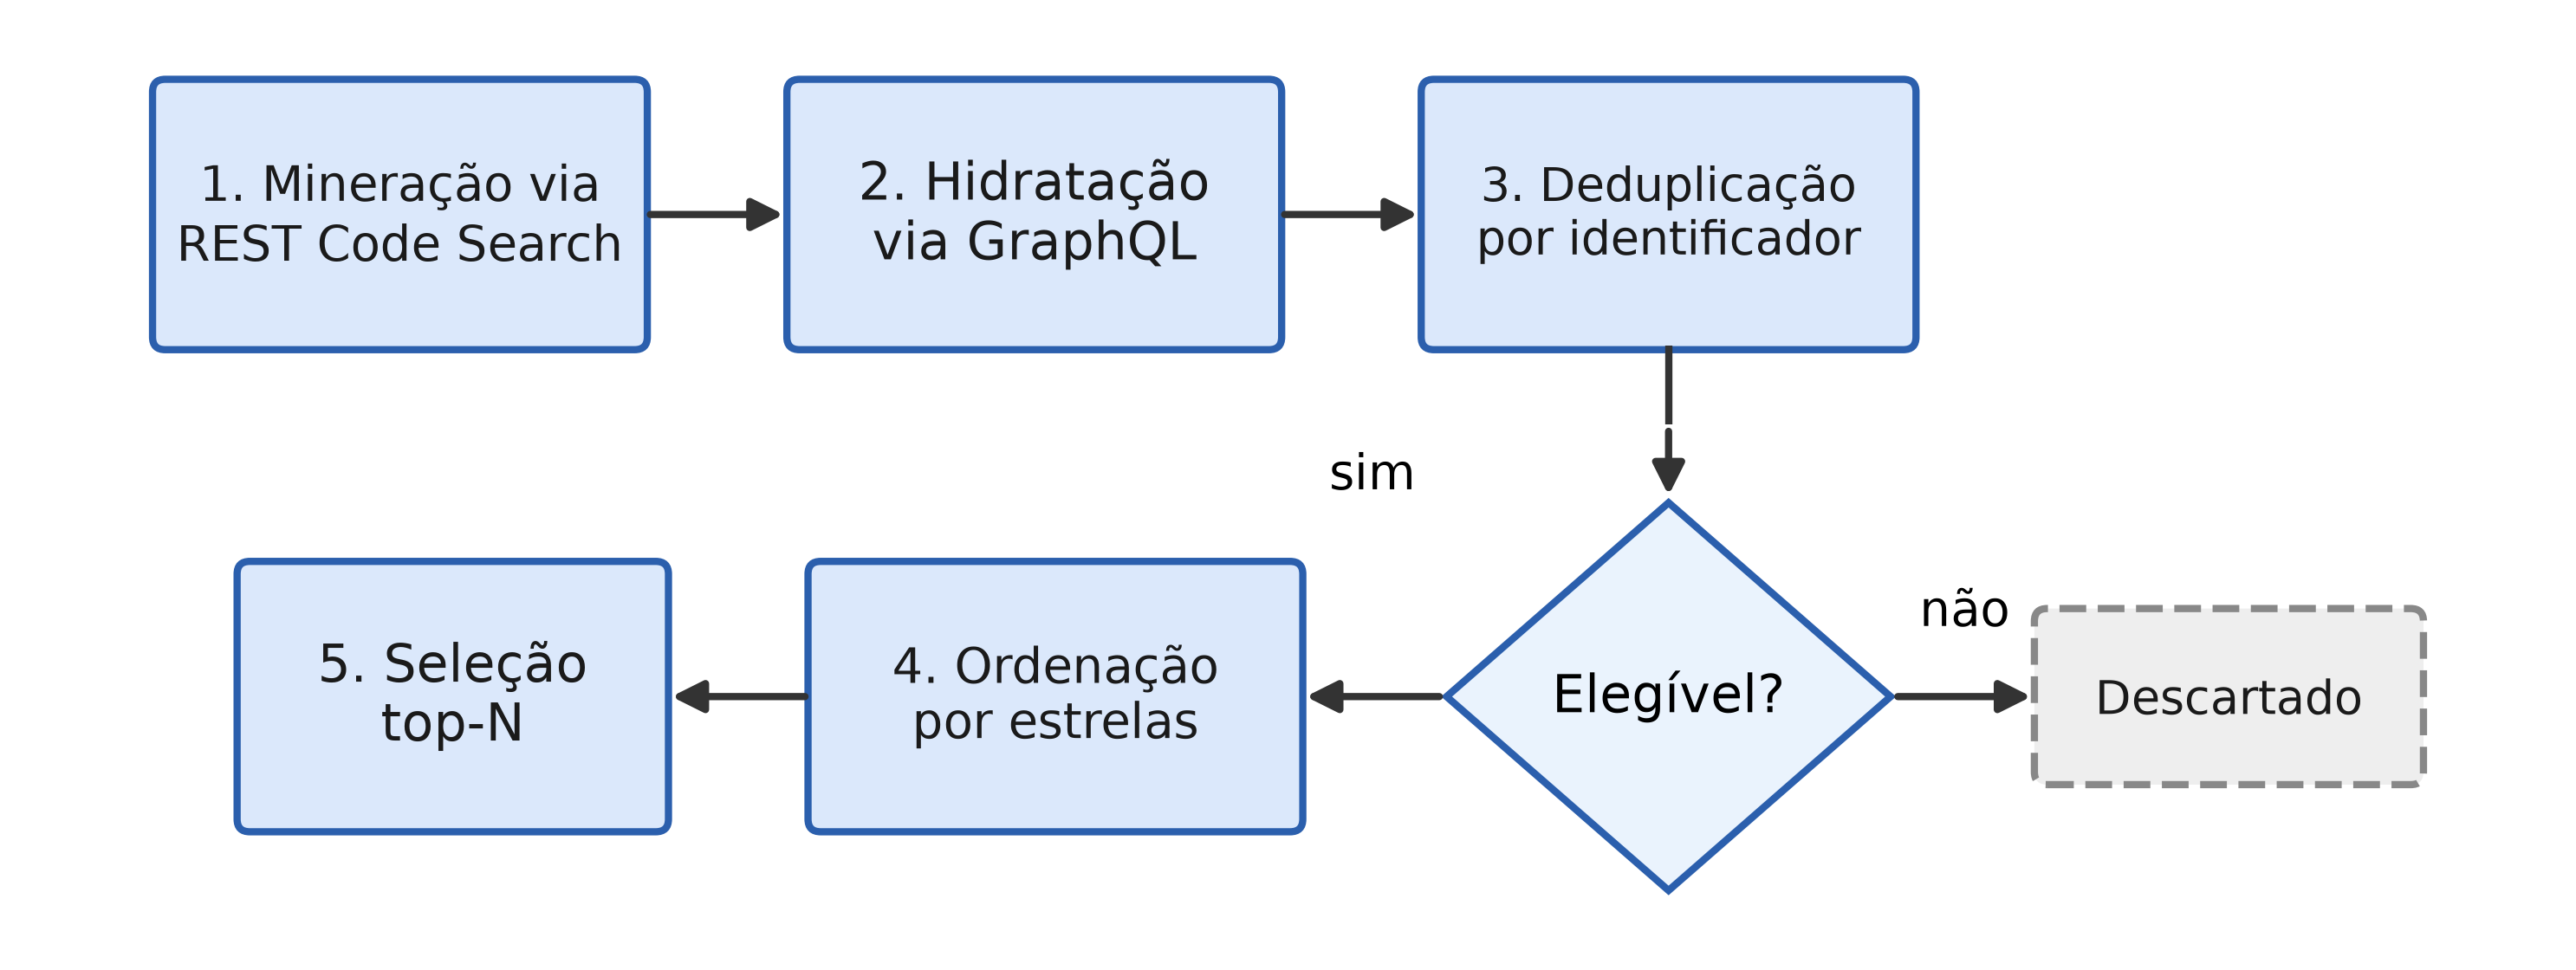
\includegraphics[width=0.5\linewidth]{./images/fluxo_etapa1_detalhado.png}
    \caption{Funcionamento detalhado da Etapa 1 (Coleta dos Repositórios)}
    \label{fig:fluxo-etapa1}
\end{figure}

A Figura~\ref{fig:fluxo-etapa1} detalha o funcionamento interno da Etapa 1.
A mineração é realizada via API REST de busca de código do GitHub,
segmentada por termos: cada combinação entre um sinal de dependência (por
exemplo, \texttt{@modelcontextprotocol/sdk}) e um arquivo de manifesto onde
esse sinal poderia estar declarado (por exemplo, \texttt{package.json})
gera uma sub-consulta independente; a linguagem não faz parte dessa
segmentação e só é determinada depois, na hidratação de cada candidato.
Cada repositório encontrado é então hidratado via GraphQL para a obtenção
de seus metadados de linguagem principal e número de estrelas, informações
não disponíveis diretamente na busca de código. Em seguida, os
repositórios são unificados por identificador (removendo duplicatas
encontradas por mais de uma sub-consulta) e submetidos a uma verificação
de elegibilidade: repositórios que são \textit{forks}, que não atingem o
piso mínimo de estrelas, ou cuja linguagem principal não está entre as
linguagens-alvo são descartados. Os repositórios aprovados são ordenados
por número de estrelas, e os mais relevantes são extraídos para compor a
amostra final.

\subsection{Etapa 2: Extração das Ferramentas}
\label{subsubsec:etapa2-detalhe}

\begin{figure}[H]
    \centering
    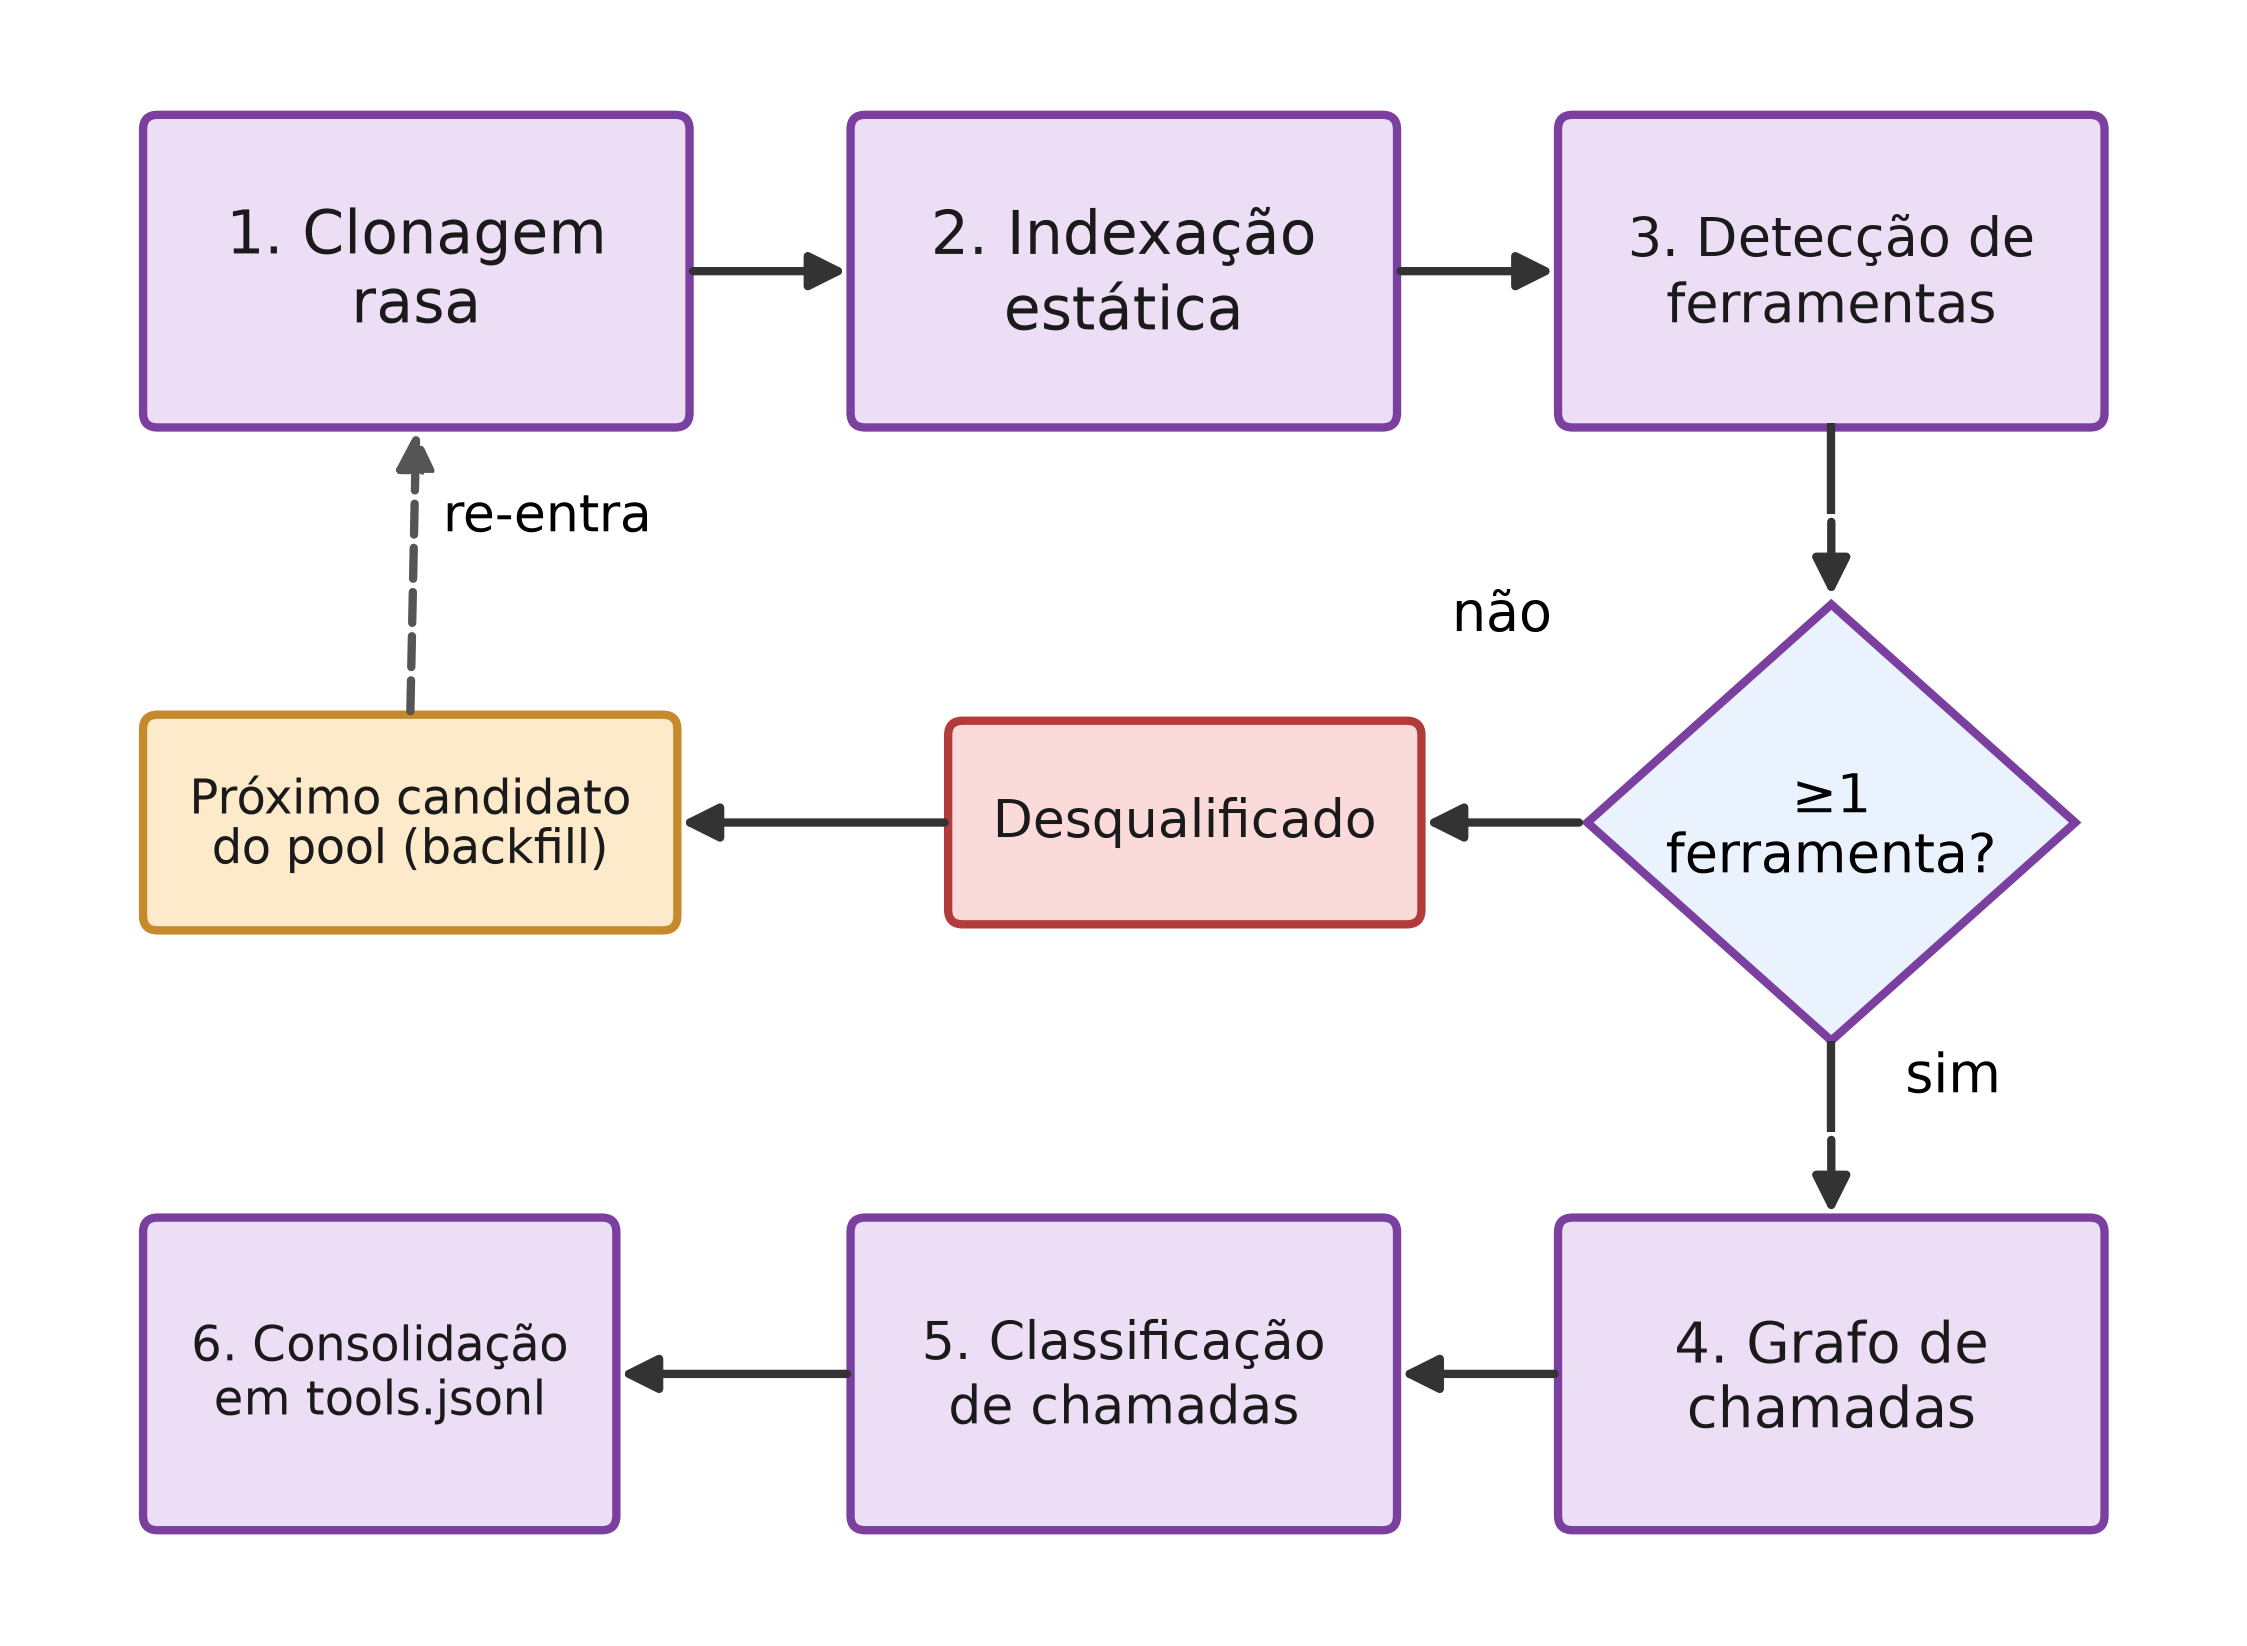
\includegraphics[width=0.5\linewidth]{./images/fluxo_etapa2_detalhado.png}
    \caption{Funcionamento detalhado da Etapa 2 (Extração das Ferramentas)}
    \label{fig:fluxo-etapa2}
\end{figure}

A Figura~\ref{fig:fluxo-etapa2} detalha o funcionamento interno da Etapa 2.
Cada repositório selecionado é primeiro clonado e então indexado
estaticamente: são catalogadas todas as definições de função/método e, por arquivo, os \textit{imports} declarados. Em seguida, aplica-se o padrão estrutural do SDK correspondente à linguagem do repositório para localizar as ferramentas declaradas. Se nenhuma ferramenta é encontrada, o repositório é desqualificado: ele é removido da seleção e substituído pelo próximo candidato ainda não tentado do \textit{pool} da Etapa 1, que reentra no mesmo fluxo a partir da clonagem — fechando um laço de preenchimento (\textit{backfill}), descrito na Seção~\ref{subsec:resultados-coleta}, que se repete até confirmar \texttt{top\_N} repositórios qualificados ou esgotar o \textit{pool}. Havendo pelo menos uma ferramenta
encontrada, um grafo de chamadas é construído para cada uma, recursivamente, a partir da função que a implementa, por uma heurística de resolução de nome, até três níveis de profundidade; cada chamada identificada é classificada como resolvida sem ambiguidade, resolvida por desempate entre candidatos ambíguos, ou externa/dinâmica (ver Apêndice~\ref{apendice:secao} para o detalhamento completo dessa heurística). Ao final, as ferramentas de cada repositório são gravadas em um arquivo próprio e, posteriormente, consolidadas em um único conjunto de dados.

\subsection{Resultados da Coleta dos Repositórios}
\label{subsec:resultados-coleta}

A coleta de repositórios da etapa 1, devolveu 12.058
candidatos brutos, todos provenientes de arquivos de dependência
(\texttt{package.json}, \texttt{pyproject.toml}, \texttt{pom.xml} e
equivalentes). A Tabela~\ref{tab:funil-coleta} apresenta o funil de atrito
aplicado sobre esse conjunto. O filtro de elegibilidade reduziu esse conjunto para 723 repositórios.
\begin{table}[H]
\centering
\caption{Funil de atrito da Etapa 1 (Coleta dos Repositórios MCP)}
\label{tab:funil-coleta}
\begin{tabular}{|p{0.6\linewidth}|r|r|}
\hline
\textbf{Etapa do filtro} & \textbf{Repositórios} & \textbf{\% do bruto} \\ \hline
Candidatos brutos (busca por manifesto) & 12.058 & 100,0\% \\ \hline
Aprovados no filtro (não-fork, estrelas $\geq$ mínimo, linguagem-alvo) & 723 & 6,0\% \\ \hline
Selecionados (qualificados pelo laço de \textit{backfill}) & 206 & 1,7\% \\ \hline
\end{tabular}
\end{table}

Diferentemente de um corte simples pelas 206 posições mais bem colocadas, a
seleção final passa por um laço de preenchimento (\textit{backfill}): um
repositório só permanece selecionado se, após a Etapa 2, confirmar pelo
menos uma ferramenta; repositórios desqualificados são substituídos pelo
próximo candidato do pool ainda não tentado, e o processo se repete até
fechar as 206 vagas ou esgotar o pool. Entre os repositórios selecionados, a distribuição por linguagem principal está longe de ser uniforme (Figura~\ref{fig:repos-linguagem}).

\begin{figure}[H]
    \centering
    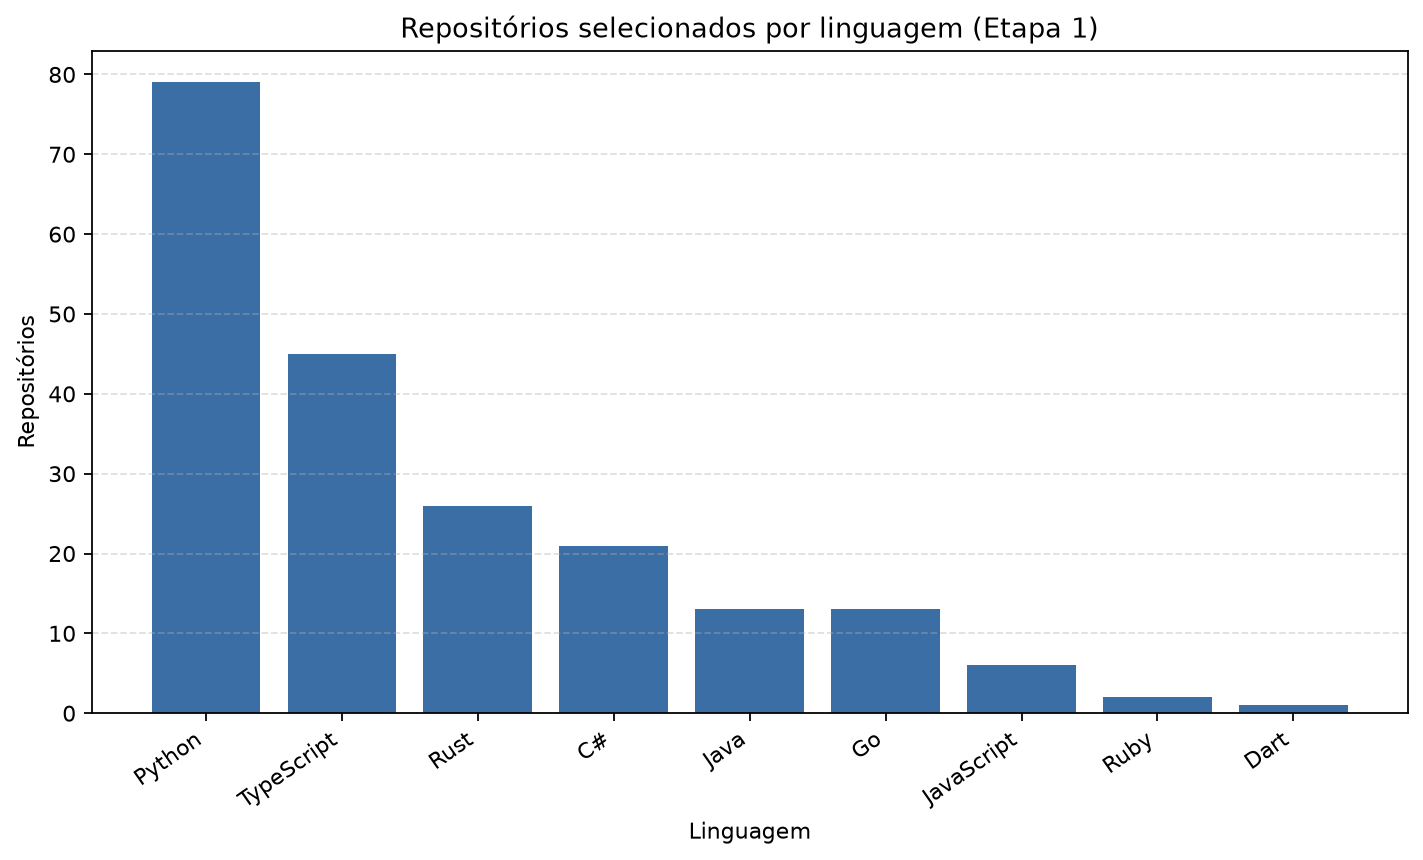
\includegraphics[width=0.8\linewidth]{./images/01_repos_por_linguagem.png}
    \caption{Repositórios selecionados por linguagem principal (Etapa 1)}
    \label{fig:repos-linguagem}
\end{figure}

Python (79, 38,3\%) e
TypeScript (45, 21,8\%) concentram 60\% da amostra, seguidos por Rust (26),
C\# (21), Java e Go (13 cada); JavaScript, Ruby e Dart somam, juntos, o
restante. Nenhum repositório em Kotlin, PHP, Elixir, Lua ou Swift
permaneceu na seleção final: os candidatos dessas linguagens que chegaram a
ser selecionados em rodadas anteriores foram descartados pelo laço de
\textit{backfill} por não confirmarem nenhuma ferramenta na Etapa 2 (ver
Seção~\ref{subsec:resultados-extracao}), ou nunca alcançaram o piso de
estrelas dentro do pool. A Figura~\ref{fig:distribuicao-estrelas} resume, em escala logarítmica, a distribuição de estrelas dos 206 repositórios selecionados.

\begin{figure}[H]
    \centering
    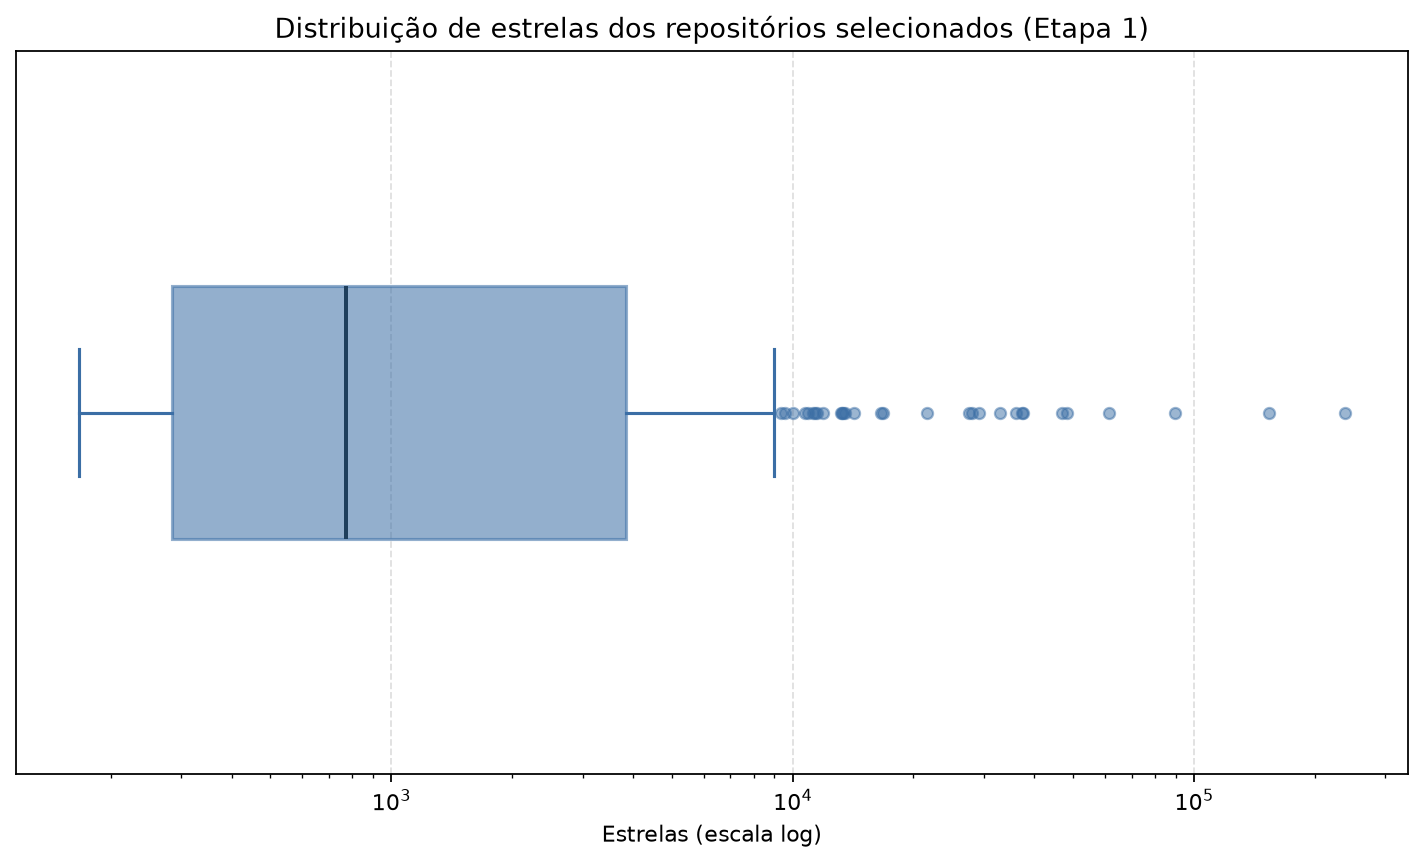
\includegraphics[width=0.6\linewidth]{./images/12_distribuicao_estrelas.png}
    \caption{Distribuição de estrelas dos 206 repositórios selecionados}
    \label{fig:distribuicao-estrelas}
\end{figure}

A distribuição é fortemente assimétrica, dominada por um pequeno número de
repositórios muito populares: a mediana (773) fica bem abaixo da média
(6.451,0), e o máximo observado, 237.449 estrelas, aparece isolado dos
demais, marcado no gráfico como valor discrepante. Já o 1º e o 3º quartis
(283 e 3.837, respectivamente) mostram que a maior parte da amostra —
inclusive o mínimo observado, 167 estrelas — se concentra numa faixa bem
mais modesta que esses extremos.

\subsection{Resultados da Extração das Ferramentas}
\label{subsec:resultados-extracao}

A Etapa 2 extraiu 12.171 ferramentas dos 206 repositórios selecionados.
Como a seleção final já incorpora o laço de \textit{backfill} descrito na
Seção~\ref{subsec:resultados-coleta}, todo repositório selecionado
confirma, por construção, pelo menos uma ferramenta; a taxa de confirmação
por linguagem é, portanto, de 100\% em todas as linguagens representadas na
amostra final, deixando de ser, sozinha, um indicador diagnóstico como seria
sob uma seleção por corte simples. A distribuição de ferramentas por linguagem (Figura~\ref{fig:tools-linguagem}) segue de perto a distribuição de repositórios vista na coleta.

\begin{figure}[H]
    \centering
    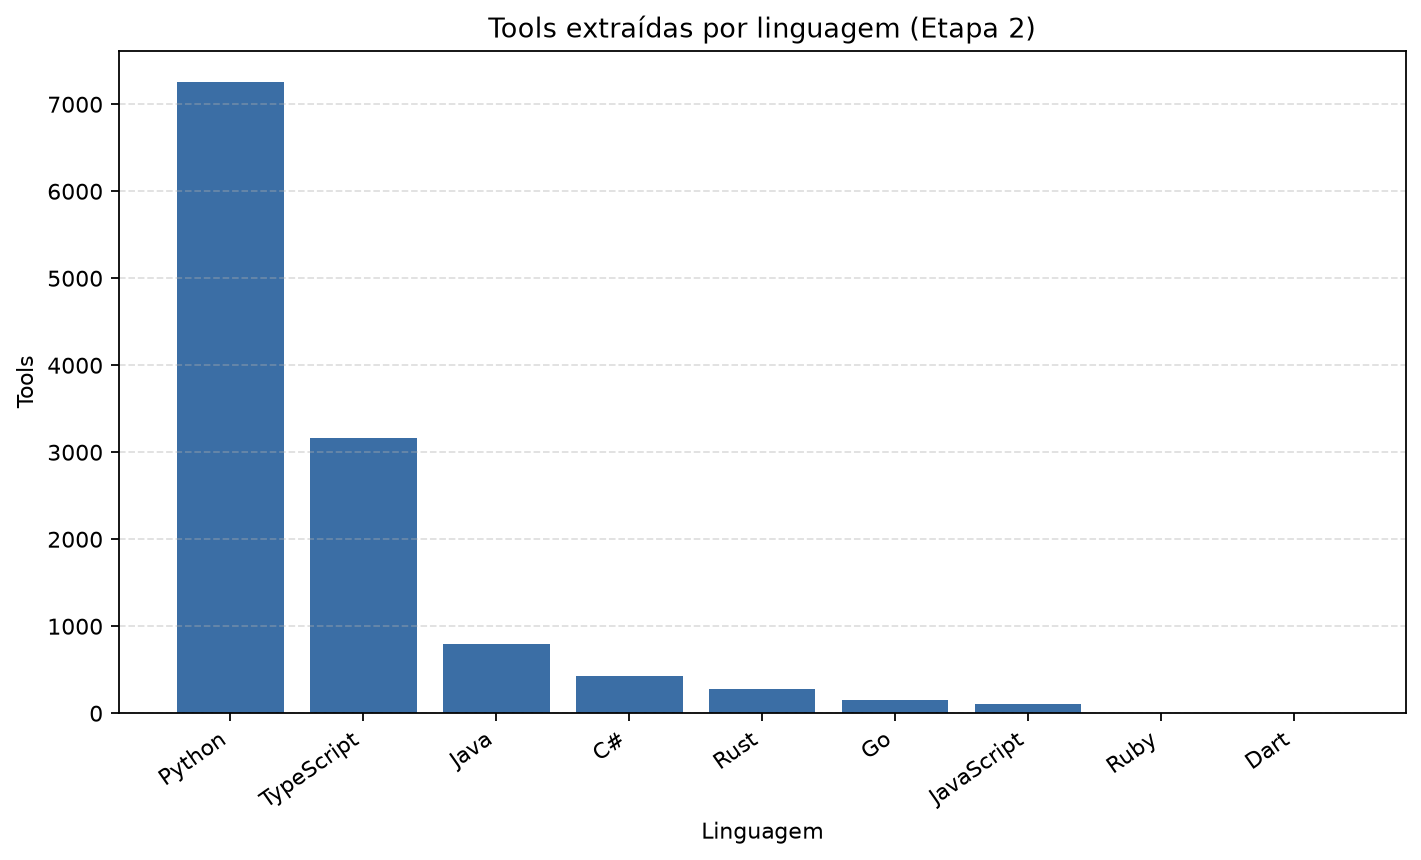
\includegraphics[width=0.8\linewidth]{./images/02_tools_por_linguagem.png}
    \caption{Ferramentas extraídas por linguagem (Etapa 2)}
    \label{fig:tools-linguagem}
\end{figure}

Python concentra 7.251 das 12.171 ferramentas (59,6\%), seguido por
TypeScript (3.162, 26,0\%) e Java (793, 6,5\%); as demais linguagens somam,
juntas, pouco mais de 7\% do total (Tabela~\ref{tab:media-tools-servidor}).

\begin{table}[H]
\centering
\caption{Repositórios selecionados e total de ferramentas extraídas, por linguagem}
\label{tab:media-tools-servidor}
\begin{tabular}{|l|r|r|r|}
\hline
\textbf{Linguagem} & \textbf{Repositórios} & \textbf{Tools (total)} & \textbf{Média/repositório} \\ \hline
Python & 79 & 7.251 & 91,78 \\ \hline
TypeScript & 45 & 3.162 & 70,27 \\ \hline
Java & 13 & 793 & 61,00 \\ \hline
C\# & 21 & 423 & 20,14 \\ \hline
Rust & 26 & 276 & 10,62 \\ \hline
Go & 13 & 149 & 11,46 \\ \hline
JavaScript & 6 & 108 & 18,00 \\ \hline
Ruby & 2 & 5 & 2,50 \\ \hline
Dart & 1 & 4 & 4,00 \\ \hline
\textbf{Total} & \textbf{206} & \textbf{12.171} & \textbf{59,08} \\ \hline
\end{tabular}
\end{table}

A concentração de ferramentas por repositório também é fortemente
assimétrica: os três repositórios com mais ferramentas respondem, sozinhos,
por 46,6\% de todo o conjunto de dados (20,4\%, 18,4\% e 7,8\%,
respectivamente) — um deles em TypeScript, os outros dois em Python. Esse
resultado eleva consideravelmente a média de ferramentas por repositório
nessas duas linguagens (Tabela~\ref{tab:media-tools-servidor}) e deve ser
considerado ao interpretar médias agregadas por linguagem nas seções
seguintes.


\begin{figure}[H]
    \centering
    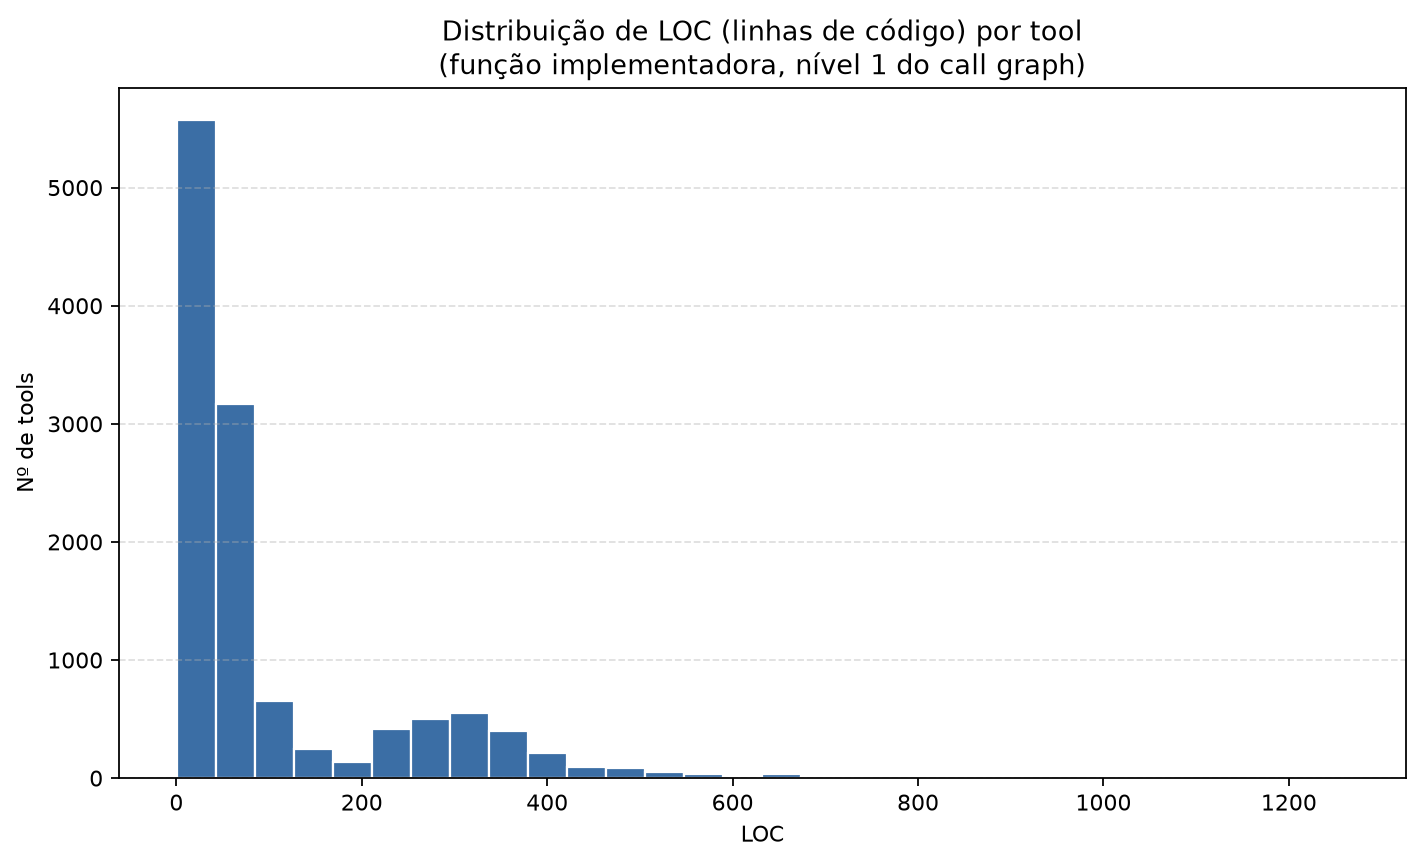
\includegraphics[width=0.8\linewidth]{./images/08_distribuicao_loc.png}
    \caption{Distribuição de LOC (linhas de código) por ferramenta, função implementadora de nível 1}
    \label{fig:loc}
\end{figure}

A Figura~\ref{fig:loc} apresenta a distribuição de linhas de código (LOC)
das funções que implementam cada ferramenta: mediana de 55 linhas e 3º
quartil de 104, contra um máximo de 1.263 linhas. Também aqui a
distribuição é assimétrica, com a maioria das implementações concentrada em
funções de porte pequeno a moderado e um número pequeno de funções bem mais
extensas.

Por fim, 94,6\% das descrições extraídas (11.512 de 12.171) correspondem a
literais de \textit{string} simples, sem necessidade de resolução
adicional; a taxa varia por linguagem, de 100\% em Dart e acima de 92\% em
Rust, TypeScript, Python, JavaScript e C\#, até 85,9\% em Java e 83,9\% em
Go. O Ruby é uma exceção notável, com apenas 40,0\% (2 de 5) de descrições
literais, ainda que sobre uma base amostral pequena.
